% --------------------------------------------------------------
% This is all preamble stuff that you don't have to worry about.
% Head down to where it says "Start here"
% --------------------------------------------------------------
 
\documentclass[12pt]{article}
 
\usepackage[margin=0.75in]{geometry} 
\usepackage{amsmath,amsthm,amssymb,mathtools,dsfont}
\usepackage{enumerate} 
\usepackage{graphicx,float} % figures
\usepackage{csvsimple,longtable,booktabs} % load csv as a table
\usepackage{listings,color} % for code snippets


%%======%%
% All this is to force LaTeX to prefix "Appendix" before a new appendix section letter
\makeatletter
% The "\@seccntformat" command is an auxiliary command
% (see pp. 26f. of 'The LaTeX Companion,' 2nd. ed.)
\def\@seccntformat#1{\@ifundefined{#1@cntformat}%
   {\csname the#1\endcsname\quad}  % default
   {\csname #1@cntformat\endcsname}% enable individual control
}
\let\oldappendix\appendix %% save current definition of \appendix
\renewcommand\appendix{%
    \oldappendix
    \newcommand{\section@cntformat}{\appendixname~\thesection\quad}
}
\makeatother
%%======%%

%%======%%
% Define for code section
\definecolor{dkgreen}{rgb}{0,0.6,0}
\definecolor{gray}{rgb}{0.5,0.5,0.5}
\definecolor{mauve}{rgb}{0.58,0,0.82}

\lstset{frame=tb,
  language=C++,
  aboveskip=3mm,
  belowskip=3mm,
  showstringspaces=false,
  columns=flexible,
  basicstyle={\scriptsize\ttfamily},
  numbers=none,
  numberstyle=\tiny\color{gray},
  keywordstyle=\color{blue},
  commentstyle=\color{dkgreen},
  stringstyle=\color{mauve},
  breaklines=true,
  breakatwhitespace=true,
  tabsize=3
}
%%======%%
%% set noindent by default and define indent to be the standard indent length
\newlength\tindent
\setlength{\tindent}{\parindent}
\setlength{\parindent}{0pt}
\renewcommand{\indent}{\hspace*{\tindent}}

\begin{document}
 
% --------------------------------------------------------------
%                         Start here
% --------------------------------------------------------------
 
\title{Assignment 4}
\author{David Fleischer\\ 
MACF 402 - Mathematical \& Computational Finance II}
 
\maketitle

\section{Question 1: {\normalfont Crude-Monte Carlo and Antithetic Variables}}

\indent Given a European put option written on an underlying asset such that $S_0 = 100, K = 40, r = 0.0175, \sigma = 0.4$, and 1 year to maturity, we have the theoretical Black-Scholes price
\begin{equation*}
	V^{BS}_P(S,K,r,\sigma,t,T) = \$0.0816128
\end{equation*}

\indent Performing simulations of the underlying asset's lognormal dynamics we are also able to determine an estimated price for the European price within a desired confidence level (95\% two-tailed confidence). Table \ref{tab:euro_call_est} shows the results of the simulation of $N$ random variates for a crude estimator and $N/2$ random variates generated for an antithetic estimator. Figures \ref{fig:call_lognormal_sim}, \ref{fig:call_CI_time}, and \ref{fig:call_eff} visualizes this information, showing the convergence towards the Black-Scholes prices for each increase in $N$. We note the consistent superiority of the antithetic estimator over the crude counterpart: The antithetic estimator shows greater estimator efficiency for a sufficiently large number of simulations.

{\footnotesize
\csvautolongtable[
      table head=\caption{Results of crude and antithetic estimation for $N$ and $N/2$ random variates generated.}\label{tab:euro_call_est}\\\hline
               \csvlinetotablerow\\\hline
               \endfirsthead\hline
               \csvlinetotablerow\\\hline
               \endhead\hline
               \endfoot,
               respect all
               ]{../data/q1_clean_estimators.csv}
}

\begin{figure}[H]
	\centering
 	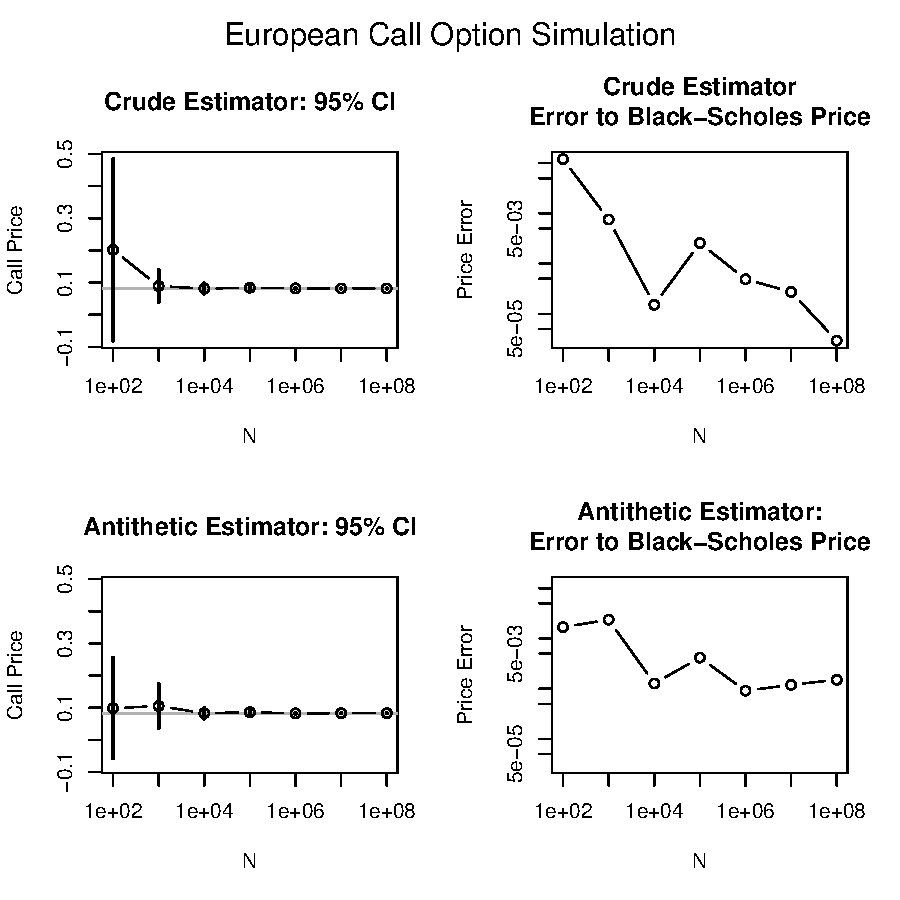
\includegraphics[scale=1]{../plots/q1/call_lognormal_sim_est.pdf}
\caption{(Top) Crude simulation of a European put option written on the asset described above. (Bottom) Antithetic simulation of the same European put option. The true (Black-Scholes) is plotted in gray. Note the convergence towards the Black-Scholes price and reduction in variance using the antithetic estimator over the crude estimator.}
\label{fig:call_lognormal_sim}
\end{figure}

\begin{figure}[H]
	\centering
 	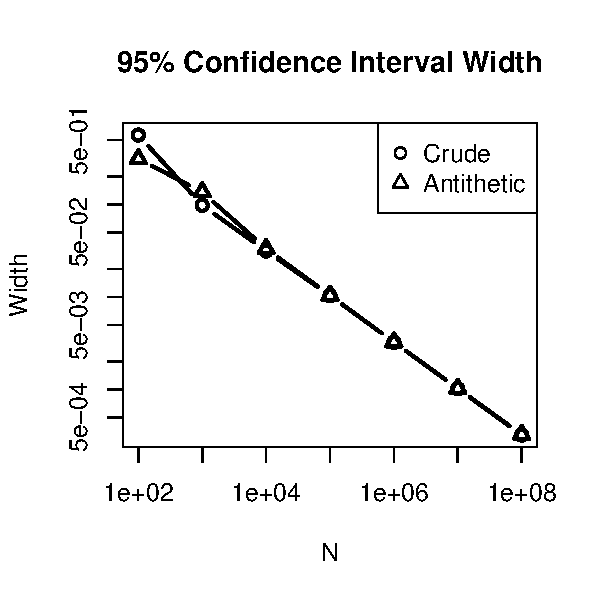
\includegraphics[scale=0.75]{../plots/q1/call_CI_widths.pdf}
	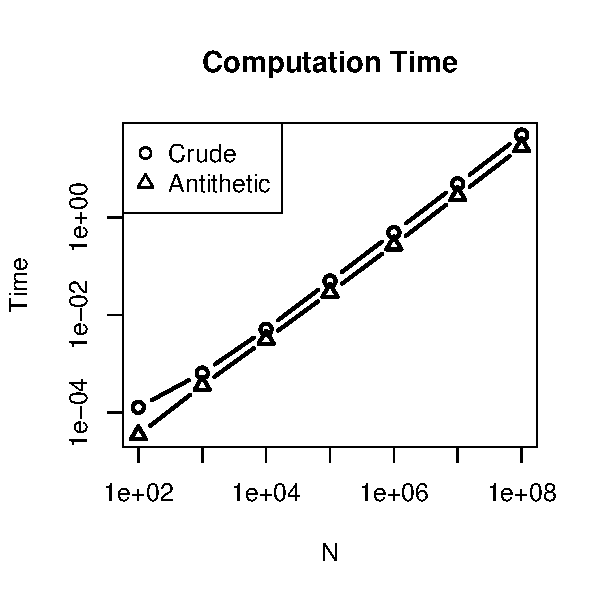
\includegraphics[scale=0.75]{../plots/q1/call_time.pdf}
\caption{European put option: (Left) Confidence intervals tighten for both crude and antithetic estimators at approximately the same (linear rate). (Right) Computation time increases linearly as a function of $N$ for both crude and antithetic estimators.}
\label{fig:call_CI_time}
\end{figure}

\begin{figure}[H]
	\centering
 	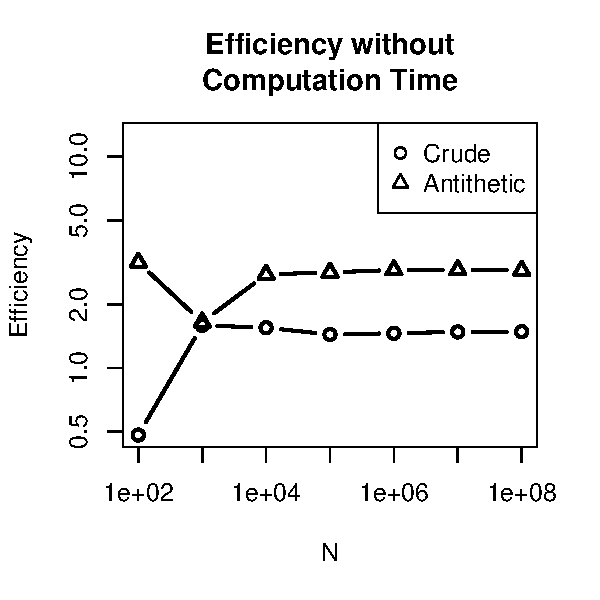
\includegraphics[scale=0.75]{../plots/q1/call_eff_wo_time.pdf}
\caption{European put option: The antithetic estimator is persistently more efficient than the crude estimator for $N$ sufficiently large.}
\label{fig:call_eff}
\end{figure}

\newpage
\section{Question 2: {\normalfont Geometric Asian Options}}

\subsection{Problem 2 (a)} Show that 

\begin{align*}
	\log \Bigg( \Bigg[ \prod^{n}_{i=1} S_{t_i} \Bigg]^{\frac{1}{n}} \Bigg) - \log S_0 &= \sum^n_{i = 1} \frac{i}{n} \Bigg[ (r - \frac{1}{2}\sigma^2) \Delta t + \sigma \sqrt{\Delta t} Z_{n - i + 1} \Bigg] \\
	&= \frac{(n + 1)}{2} (r - \frac{1}{2}\sigma^2)\Delta t + \sum^n_{i = 1}\sigma_i Z_i
\end{align*}

where $\{Z_i\}^n_{i=1}$ are i.i.d. standard normal random variables and $\sigma_i = \frac{i}{n}\sigma\sqrt{\Delta t}$. \\

{\bf Solution 2 (a)}. We have that
\begin{align*}
	S_{t_1} &= S_0 e^{ (\cdots) } \\
	S_{t_2} = S_{t_1}e^{ (\cdots) } &= S_0 e^{ (\cdots) } e^{ (\cdots) } \\
	S_{t_3} = S_{t_2}e^{ (\cdots) } &= S_0 e^{ (\cdots) } e^{ (\cdots) } e^{ (\cdots) } \\	
	\vdots \\
	S_{t_n} &= S_0 \prod^n_{i = 1} e^{(\cdots)}	
\end{align*}

We recognize that the number of exponential terms is $\sum^n_{i = 1} i = \frac{n(n + 1)}{2}$. Hence
\begin{align*}
	\left[ \prod^n_{i = 1} S_{t_i} \right]^\frac{1}{n} &= \left[ S_0^n \prod^\frac{n(n + 1)}{2}_{i = 1} e^{ \left( r - \frac{1}{2}\sigma^2 \right)\Delta t + \sigma\sqrt{\Delta t}Z_i } \right]^\frac{1}{n} \\
	&= S_0 \exp \left[\frac{1}{n} \sum^\frac{n(n + 1)}{2}_{i = 1} \left( r - \frac{1}{2}\sigma^2 \right)\Delta t + \sigma\sqrt{\Delta t} Z_i \right]
\end{align*}

So,
\begin{align*}
	\log \left( \left[ \prod^n_{i = 1} S_{t_i} \right]^\frac{1}{n} \right) &= \log S_0 + \frac{1}{n} \sum^\frac{n(n + 1)}{2}_{i = 1} \left( r - \frac{1}{2}\sigma^2 \right)\Delta t + \sigma\sqrt{\Delta t} Z_i \\
	&=  \log S_0 + \frac{1}{n}\frac{ n(n + 1) }{2}\left( r - \frac{1}{2}\sigma^2 \right)\Delta t + \frac{1}{n} \sum^\frac{n(n + 1)}{2}_{i = 1} \sigma\sqrt{\Delta t} Z_i \\
	&=  \log S_0 + \frac{ (n + 1) }{2}\left( r - \frac{1}{2}\sigma^2 \right)\Delta t + \frac{1}{n} \sum^\frac{n(n + 1)}{2}_{i = 1} \sigma\sqrt{\Delta t} Z_i \\
\end{align*}

From properties of the normal distribution we note that
\begin{align*}
	\sum^\frac{n(n + 1)}{2}_{i = 1} \sigma\sqrt{\Delta t} Z_i &\sim N\left( 0, \sum^\frac{n(n + 1)}{2}_{i = 1} \sigma^2\Delta t \right) \\
	&\sim N\left( 0, \frac{ n(n + 1) }{2} \sigma^2\Delta t \right) \\
	&\sim N \left(0, \sum^n_{i = 1} i \sigma^2\Delta t \right) \\
	&\sim \sum^n_{i = 1} i\sigma\sqrt{\Delta t} Z_i
\end{align*}

Thus,
\begin{align*}
	\log \left( \left[ \prod^n_{i = 1} S_{t_i} \right]^\frac{1}{n} \right) &= \log S_0 + \frac{ (n + 1) }{2}\left( r - \frac{1}{2}\sigma^2 \right)\Delta t + \frac{1}{n} \sum^\frac{n(n + 1)}{2}_{i = 1} \sigma\sqrt{\Delta t} Z_i \\
	&= \log S_0 + \frac{ (n + 1) }{2}\left( r - \frac{1}{2}\sigma^2 \right)\Delta t + \frac{1}{n} \sum^n_{i = 1} i\sigma\sqrt{\Delta t} Z_i 
\end{align*}

Letting $\sigma_i := \frac{i}{n}\sigma\sqrt{\Delta t}$ we have
\begin{equation*}
	\log \left( \left[ \prod^n_{i = 1} S_{t_i} \right]^\frac{1}{n} \right) - \log S_0 = \frac{ (n + 1) }{2}\left( r - \frac{1}{2}\sigma^2 \right)\Delta t + \sum^n_{i = 1} \sigma_i Z_i
\end{equation*}

as desired.

%{\bf Solution 2 (a)}. With It\^{o}'s rule in $n$ spatial dimensions we have
%\begin{align*}
%	f(t, X^{(1)}_t, X^{(2)}_t, ..., X^{(n)}_t) = f(0, X^{(1)}_0, X^{(2)}_0, ..., X^{(n)}_0) + \int^t_0 f_t(u,X^{(1)}_u, X^{(2)}_u, ..., X^{(n)}_u) \,du \\
%	\hphantom{{}={}} + \sum^n_{i=1} \int^t_0 f_{X^{(i)}}(u,X^{(1)}_u, X^{(2)}_u, ..., X^{(n)}_u) \,dX^{(i)}_u \\
%	\hphantom{{}={}} + \frac{1}{2} \sum^n_{i=1} \sum^n_{j=1} \int^t_0 f_{X^{(i)}X^{(j)}}(u,X^{(1)}_u, X^{(2)}_u, ..., X^{(n)}_u) \,d\langle X^{(i)}_{(\cdot)}, X^{(j)}_{(\cdot)}\rangle_u
%\end{align*}
%
%Letting $f(t, x_1, x_2, ..., x_n) = \log \Big( \Big[ \prod^{n}_{i=1} x_i \Big]^{\frac{1}{n}} \Big)$ we compute our derivatives
%\begin{align*}
%	f_{x_i} &= \frac{\partial}{\partial x_i} \log \Bigg( \Bigg[ \prod^{n}_{j=1} x_j \Bigg]^{\frac{1}{n}} \Bigg) \\
%	&= \frac{1}{\Big( \prod^{n}_{j=1} x_j \Big)^{\frac{1}{n}} } \cdot \frac{\partial}{\partial x_i} \Big( \prod^{n}_{j=1} x_j \Big)^{\frac{1}{n}} \\
%	&= \frac{1}{\Big( \prod^{n}_{j=1} x_j \Big)^{\frac{1}{n}} } \cdot \frac{ \Big( \prod^{n}_{j=1} x_j \Big)^{\frac{1}{n} - 1} }{n} \cdot \frac{\partial}{\partial x_i} \prod^{n}_{i=1} x_j \\
%	&= \frac{1}{\Big( \prod^{n}_{j=1} x_j \Big)^{\frac{1}{n}} } \cdot \frac{ \Big( \prod^{n}_{j=1} x_j \Big)^{\frac{1}{n} - 1} }{n} \cdot \prod^{n}_{j\neq i} x_j \\
%	&= \frac{1}{n} \cdot \frac{ \Big( \prod^{n}_{j=1} x_j \Big)^{\frac{1}{n}} \Big( \prod^{n}_{j=1} x_j \Big)^{-1} }{\Big( \prod^{n}_{j=1} x_j \Big)^{\frac{1}{n}} } \cdot \prod^{n}_{j\neq i} x_j  \\
%	&= \frac{ \prod^{n}_{j\neq i} x_j }{ n\prod^{n}_{j=1} x_j } = \frac{1}{nx_i}
%\end{align*}
%
%and
%\begin{equation*}
%	f_{x_ix_j} = \begin{cases}
%		\frac{\partial}{\partial x_j} \frac{1}{nx_i} = 0 & i \neq j \\
%		\frac{\partial}{\partial x_i} \frac{1}{nx_i} = -\frac{1}{nx_i^2} & i = j
%	\end{cases}
%\end{equation*} 
%
%So, using It\^{o}'s rule with $x_i = (B_{t_i} - B_{t_{i-1}}) = \sqrt{\Delta t}Z_i$ with $Z_i \sim N(0,1)$, we get
%\begin{align*}
%	f(t, S_{t_1}, S_{t_2}, ... , S_{t_n}) &= f(0, S_0, S_0, ..., S_0) + \int^t_0 f_t(u, S_{t_1}, S_{t_2}, ..., S_{t_n}) \,du \\
%	&\hphantom{{}={f(0, S_0, S_0, ..., S_0) + \int^t_0}} + \sum^n_{i=1} \int^t_0  f_{x_i}(u, S_{u_1}, S_{u_2}, ..., S_{u_n}) \,dS_{u_i} \\
%	&\hphantom{{}={f(0, S_0, S_0, ..., S_0) + \int^t_0}} + \frac{1}{2} \sum^n_{i=1} \int^t_0 f_{x_ix_i}(u, S_{u_1}, S_{u_2}, ..., S_{u_n}) \,d\langle S_{(\cdot)} \rangle_{u_i} \\
%	\implies  \log \Bigg( \Bigg[ \prod^{n}_{i=1} S_{t_i} \Bigg]^{\frac{1}{n}} \Bigg) &= \log \Bigg( \Bigg[ \prod^{n}_{i=1} S_{0} \Bigg]^{\frac{1}{n}} \Bigg) + \sum^n_{i = 0} \int^{t_i}_0 \frac{1}{nS_{u_i}} \,dS_{u_i} - \frac{1}{2} \sum^n_{i=1} \int^{t_i}_0 \frac{1}{nS_{u_i}^2}  \,d\langle S_{(\cdot)} \rangle_{u_i} \\
%	&= \log S_0 + \sum^n_{i = 0} \int^{t_i}_0 \frac{1}{nS_{u_i}} \,dS_{u_i} - \frac{1}{2} \sum^n_{i=1} \int^{t_i}_0 \frac{1}{nS_{u_i}^2}  \,d\langle S_{(\cdot)} \rangle_{u_i}  
%\end{align*}
%
%We have differential and quadratic variation terms
%\begin{align*}
%	dS_t &= rS_t\,dt + \sigma S_t \,dB_t \\
% 	\implies d\langle S_{(\cdot)}\rangle_u &= \sigma^2S_t^2 \,dt
%\end{align*}
%
%So
%\begin{align*}
%	 \log \Bigg( \Bigg[ \prod^{n}_{i=1} S_{t_i} \Bigg]^{\frac{1}{n}} \Bigg) &= \log S_0 +   \sum^n_{i = 1} \int^{t_i}_0 \frac{1}{nS_{u_i}} \big( rS_{u_i}\,du_i + \sigma S_{u_i} \,dB_{u_i} \big) - \frac{1}{2} \sum^n_{i=1} \int^{t_i}_0 \frac{1}{nS_{u_i}^2} \sigma^2S_{u_i}^2 \,du_i \\
%	 &= \log S_0 + \sum^n_{i = 1} \Bigg[ \int^{t_i}_0 \frac{r}{n}\,du_i + \int^{t_i}_0 \frac{\sigma}{n}\,dB_{u_i} \Bigg] - \frac{1}{2} \sum^n_{i=1} \int^{t_i}_0 \frac{\sigma^2}{n} \,du_i \\ 
% 	 &= \log S_0 + \sum^n_{i = 1} \frac{1}{n} \Bigg[ \int^{t_i}_0 \Big( r - \frac{1}{2}\sigma^2 \Big) \,du_i + \int^{t_i}_0 \sigma\,dB_{u_i} \Bigg]\\  
%	&= \log S_0 + \sum^n_{i = 0} \frac{1}{n} \bigg[ \Big(r - \frac{1}{2}\sigma^2 \Big)t_i + \sigma B_{t_i} \bigg] \\
%	&= \log S_0 + \sum^n_{i = 0} \frac{1}{n} \bigg[ \Big(r - \frac{1}{2}\sigma^2 \Big)t_i + \sigma \sqrt{t_i}Z_i \bigg], \quad \{Z_i\}^n_{i=1} \text{ i.i.d. } N(0,1) 
%\end{align*}
%
%But $t_i \equiv i\Delta t$, so
%\begin{align*}
%	\log \Bigg( \Bigg[ \prod^{n}_{i=1} S_{t_i} \Bigg]^{\frac{1}{n}} \Bigg) &= \log S_0 + \sum^n_{i = 0} \frac{1}{n} \bigg[ \Big(r - \frac{1}{2}\sigma^2 \Big)i\Delta t + \sigma \sqrt{i\Delta t}Z_i \bigg] \\
%	&= \log S_0 + \sum^n_{i = 0} \frac{i}{n} \bigg[ \Big(r - \frac{1}{2}\sigma^2 \Big)\Delta t + \sigma \sqrt{\Delta t}Z_i \bigg] \\
%	&= \log S_0 + \frac{(n + 1)}{2} \Big(r - \frac{1}{2}\sigma^2 \Big)\Delta t +  \sum^n_{i = 0} \frac{i}{n} \sigma \sqrt{\Delta t}Z_i 
%\end{align*}
%
%Letting $\sigma_i = \frac{i}{n}\sigma\sqrt{\Delta t}$, we rearrange our equation to yield
%\begin{equation*}
%	\log \Bigg( \Bigg[ \prod^{n}_{i=1} S_{t_i} \Bigg]^{\frac{1}{n}} \Bigg) - \log S_0 = \frac{(n + 1)}{2} \Big(r - \frac{1}{2}\sigma^2 \Big)\Delta t +  \sum^n_{i = 0} \sigma_iZ_i 
%\end{equation*}
%
%as desired. \\

\subsection{Problem 2 (b)} Show that $\log \Big( \big[ \prod^{n}_{i=1} S_{t_i} \big]^{\frac{1}{n}} \Big) - \log S_0$ has normal distribution with mean
\begin{equation*}
	(r - \frac{1}{2}\sigma^2)\frac{(n + 1)}{2n}T
\end{equation*}

and variance
\begin{equation*}
	\frac{\sigma^2(n + 1)(2n + 1)}{6n^2} T
\end{equation*}

{\bf Solution 2 (b)}. We have that
\begin{equation*}
	\log \Bigg( \Bigg[ \prod^{n}_{i=1} S_{t_i} \Bigg]^{\frac{1}{n}} \Bigg) - \log S_0 = \frac{(n + 1)}{2} \Big(r - \frac{1}{2}\sigma^2 \Big)\Delta t +  \sum^n_{i = 0} \sigma_iZ_i 
\end{equation*}

Thus
\begin{align*}
	\mathbb E \Bigg[ \log \Bigg( \Bigg[ \prod^{n}_{i=1} S_{t_i} \Bigg]^{\frac{1}{n}} \Bigg) - \log S_0 \Bigg] &= \mathbb E \Bigg[ \frac{(n + 1)}{2} \Big(r - \frac{1}{2}\sigma^2 \Big)\Delta t +  \sum^n_{i = 0} \sigma_iZ_i \Bigg] \\
	&= \frac{(n + 1)}{2} \Big(r - \frac{1}{2}\sigma^2 \Big)\Delta t + \sum^n_{i = 0} \sigma_i\mathbb E [ Z_i ] \quad \text{(by linearity)}
\end{align*}

but $Z_i \sim N(0,1) \implies \mathbb E[Z_i] = 0$, hence
\begin{equation*}
	\mathbb E \Bigg[ \log \Bigg( \Bigg[ \prod^{n}_{i=1} S_{t_i} \Bigg]^{\frac{1}{n}} \Bigg) - \log S_0 \Bigg] = \frac{(n + 1)}{2} \Big(r - \frac{1}{2}\sigma^2 \Big)\Delta t 
\end{equation*}

We have that $n\Delta t = T \iff \Delta t = \frac{T}{n}$, thus
\begin{align*}
	\mathbb E \Bigg[ \log \Bigg( \Bigg[ \prod^{n}_{i=1} S_{t_i} \Bigg]^{\frac{1}{n}} \Bigg) - \log S_0 \Bigg] &= \frac{(n + 1)}{2} \Big(r - \frac{1}{2}\sigma^2 \Big)\frac{T}{n} \\
	&= \Big(r - \frac{1}{2}\sigma^2 \Big)\frac{(n + 1)}{2n}T
\end{align*}

as desired. Now, for the variance, we use the identity $\mathrm{Var}[X] = \mathbb E[X^2] - \mathbb E^2[X]$. Computing these terms we get
\begin{equation*}
	\mathbb E^2[X] = \mathbb E^2 \Bigg[ \log \Bigg( \Bigg[ \prod^{n}_{i=1} S_{t_i} \Bigg]^{\frac{1}{n}} \Bigg) - \log S_0 \Bigg] = \bigg( \Big(r - \frac{1}{2}\sigma^2 \Big)\frac{(n + 1)}{2n}T \bigg)^2
\end{equation*}

and
\begin{align*}
	\mathbb E[X^2] &= \mathbb E \Bigg[ \Bigg( \log \Bigg( \Bigg[ \prod^{n}_{i=1} S_{t_i} \Bigg]^{\frac{1}{n}} \Bigg) - \log S_0 \Bigg)^2 \Bigg] =  \mathbb E \Bigg[ \Bigg( \frac{(n + 1)}{2} \Big(r - \frac{1}{2}\sigma^2 \Big)\Delta t +  \sum^n_{i = 0} \sigma_iZ_i \Bigg)^2 \Bigg] \\
	&= \mathbb E\Bigg[ \bigg(\frac{(n + 1)}{2} \Big(r - \frac{1}{2}\sigma^2 \Big)\Delta t\bigg)^2 + \frac{(n + 1)}{2} \Big(r - \frac{1}{2}\sigma^2 \Big)\Delta t \sum^n_{i = 0} \sigma_iZ_i + \bigg(\sum^n_{i = 0} \sigma_iZ_i \bigg)^2 \Bigg] \\
	&= \bigg(\frac{(n + 1)}{2} \Big(r - \frac{1}{2}\sigma^2 \Big)\Delta t\bigg)^2 + \frac{(n + 1)}{2} \Big(r - \frac{1}{2}\sigma^2 \Big)\Delta t \sum^n_{i = 0}\sigma_i \mathbb E \big[Z_i\big] + \mathbb E \Bigg[ \bigg(\sum^n_{i = 0} \sigma_iZ_i \bigg)^2 \Bigg] \\
	&= \bigg(\frac{(n + 1)}{2} \Big(r - \frac{1}{2}\sigma^2 \Big)\Delta t\bigg)^2 + \mathbb E \Bigg[ \bigg(\sum^n_{i = 0} \sigma_iZ_i \bigg)^2 \Bigg]	
\end{align*}

Thus, we see that the $\Big(\frac{(n + 1)}{2} \big(r - \frac{1}{2}\sigma^2 \big)\Delta t\Big)^2$ terms cancel and are left with
\begin{align*}
	\mathrm{Var} \Bigg[ \log \Bigg( \Bigg[ \prod^{n}_{i=1} S_{t_i} \Bigg]^{\frac{1}{n}} \Bigg) - \log S_0 \Bigg] &= \mathbb E \Bigg[ \bigg(\sum^n_{i = 0} \sigma_iZ_i \bigg)^2 \Bigg] \\
	&= \mathbb E \Bigg[ \bigg(\sum^n_{i = 0} X_i \bigg)^2 \Bigg] \quad \text{for } X_i \sim N(0, \sigma_i^2)
\end{align*}

To compute this term we use the result that
\begin{equation*}
	\sum^n_{i=1} X_i \sim N \bigg(0, \sum^n_{i=1}\sigma^2_i \bigg)
\end{equation*}

and for $X \sim N(0, \sigma^2)$ we also have the result that
\begin{equation*}
	\mathbb E[X^n] = \begin{cases}
		0 & n \text{ odd} \\
		1 \cdot 3 \cdot \cdots (n - 3) \cdot (n - 1) \cdot \sigma^{\frac{n}{2}} & n \text{ even}
	\end{cases}
\end{equation*}

Thus,
\begin{align*}
	\mathrm{Var} \Bigg[ \log \Bigg( \Bigg[ \prod^{n}_{i=1} S_{t_i} \Bigg]^{\frac{1}{n}} \Bigg) - \log S_0 \Bigg] = \mathbb E \bigg[ \bigg(\sum^n_{i=1} X_i \bigg)^2\bigg] &= \sum^n_{i=1}\sigma^2_i \\
	&= \bigg( \sum^n_{i=1} \frac{i}{n}\sigma\sqrt{\Delta t} \bigg)^2 \\
	&= \sigma^2 \Delta t \sum^n_{i=1} \frac{i^2}{n^2} \\
	&= \sigma^2 \Delta t \frac{n (n+1) (2n + 1)}{6n^2} \\
	&= \frac{\sigma^2 (n+1) (2n + 1)}{6n^2} T
\end{align*}

as desired. \\

\subsection{Problem 2 (c)} 

\indent Show that the time-zero price of the time-$T$ expiry geometric average Asian call option with strike price $K$ is
\begin{equation*}
	C^{GA}_0 = e^{-rT} \Big( S_0 e^{\hat{\mu}T}\Phi(\hat{d}_1) - K\Phi(\hat{d}_2) \Big)
\end{equation*}

where 
\begin{align*}
	&\hat{\mu} = \Big(r - \frac{1}{2}\sigma^2 \Big)\frac{(n + 1)}{2n} + \frac{1}{2}\hat{\sigma}^2, \quad \hat{\sigma}^2 = \frac{\sigma^2 (n + 1)(2n + 1)}{6n^2} \\
	&\hat{d}_1 = \frac{\log \frac{S_0}{K} + (\hat{\mu} + \frac{1}{2}\hat{\sigma}^2)T}{\hat{\sigma}\sqrt{T}} \\
	&\hat{d}_2 = \hat{d}_1 - \hat{\sigma}\sqrt{T}
\end{align*}

{\bf Solution 2 (c)}. We note that

\begin{align*}
	\frac{S_{t_i}}{S_{t_{i - 1}}} &= \frac{S_{t_{i - 1}} e^{ (r - \frac{1}{2}\sigma^2)\Delta t + \sigma (B_{t_{i - 1}} - B_{t_{i - 2}}) } }{ S_{t_{i - 1}} } \\
	&= e^{ (r - \frac{1}{2}\sigma^2) \Delta t +  \sigma (B_{t_i} - B_{t_{i - 1}}) } \\
	\implies \log \frac{S_{t_i}}{S_{t_{i - 1}}} &= \left(r - \frac{1}{2}\sigma^2\right)\Delta t + \sigma \left( B_{t_i}  - B_{t_{i - 1}} \right) \\
	\implies \log \frac{S_{t_i}}{S_{t_{i - 1}}} &\sim N\left( \left(r - \frac{1}{2}\sigma^2\right)\Delta t, \sigma^2\Delta t \right)
\end{align*}

Thus
\begin{align*}
\left[ \prod^n_{i=1} S_{t_i} \right]^{\frac{1}{n}} &= \left[S_0^{n} \frac{S_{t_1}^n}{S_0^n} \frac{S_{t_2}^{n - 1}}{S_{t_1}^{n - 1}} \cdots \frac{S_{t_{n - 1}}^{2}}{S_{t_{n - 2}}^2} \frac{S_{t_n}}{S_{t_{n - 1}}} \right]^\frac{1}{n} \\
	&= S_0 \left[ \frac{S_{t_1}^n}{S_0^n} \frac{S_{t_2}^{n - 1}}{S_{t_1}^{n - 1}} \cdots \frac{S_{t_{n - 1}}^{2}}{S_{t_{n - 2}}^2} \frac{S_{t_n}}{S_{t_{n - 1}}} \right]^\frac{1}{n}
\end{align*}

Letting $ X_i = \log \frac{S_{t_i}}{S_{t_{i - 1}}}$ we have $\left[ \left( \frac{S_{t_i}}{S_{t_{i - 1}}}\right)^k \right]^\frac{1}{n} = \exp \left[ \left(\frac{k}{n}\right) X_i \right]$, so
\begin{align*}
	\left[ \prod^n_{i=1} S_{t_i} \right]^{\frac{1}{n}} &= S_0 \exp\left[\left(\frac{n}{n}\right) X_1 + \left(\frac{n - 1}{n}\right) X_2 + \cdots + \left(\frac{2}{n}\right) X_{n - 1} + \left(\frac{1}{n}\right) X_n  \right] \\
	&= S_0 \exp\left[ 	\frac{1}{n} \sum^n_{k = 1} (n - k + 1)X_k  \right]
\end{align*}

But
\begin{align*}
	\sum^n_{k = 1} (n - k + 1)X_k &= n^2\sum^n_{k=1}X_k - \frac{n(n + 1)}{2}\sum^n_{k=1}X_k + n\sum^n_{k=1}X_k \\
	&= \left[n - \frac{(n + 1)}{2}+ 1 \right]n\sum^n_{k=1}X_k \\
	&= \left[ \frac{2n - (n + 1) + 2}{2} \right] n\sum^n_{k=1}X_k \\
	&= \frac{n(n + 1)}{2}\sum^n_{k=1}X_k \\
	&= \sum^n_{k = 1} kX_k
\end{align*}

Thus,
\begin{align*}
	\left[ \prod^n_{i=1} S_{t_i} \right]^{\frac{1}{n}} &= S_0 \exp\left[ 	\frac{1}{n} \sum^n_{k = 1} (n - k + 1)X_k  \right] \\
	&= S_0 \exp \left[ \frac{1}{n} \sum^n_{k=1}kX_k \right]
\end{align*}

Recalling that $X_i \sim N\left( \left(r - \frac{1}{2}\sigma^2\right)\Delta t, \sigma^2\Delta t \right)$ we use the result that, for $W_i \sim N(\mu_i, \sigma^2_i)$ and $c_i \in \mathbb R$,
\begin{equation*}
	\sum^n_{i=1} c_iW_i \sim N \bigg( \sum^n_{i = 1} c_i\mu_i, \sum^n_{i = 1}c_i^2\sigma^2_i \bigg) 
\end{equation*}

Hence
\begin{align*}
	\frac{1}{n} \sum^n_{k = 1} kX_k &\sim N\left( \frac{1}{n}\left(r - \frac{1}{2}\sigma^2\right)\Delta t \sum^n_{k = 1} k, \frac{1}{n^2}\sigma^2\Delta t \sum^n_{k = 1} k^2 \right) \\
	&\sim N \left( \frac{1}{n}\left(r - \frac{1}{2}\sigma^2\right)\Delta t\frac{(n + 1)}{2}, \frac{1}{n^2}\sigma^2\Delta t \frac{n(n + 1)(2n + 1)}{6}\right)
\end{align*}

But $\Delta t \equiv \frac{T}{n}$, so
\begin{align*}
	\frac{1}{n}\sum^n_{k = 1} kX_k &\sim N\left( \left(r - \frac{1}{2}\sigma^2\right)\frac{(n + 1)}{2n}T, \frac{\sigma^2(n + 1)(2n + 1)}{6n^2}T \right) \\
	\implies \frac{1}{n} \sum^n_{k = 1} kX_k &= \left(r - \frac{1}{2}\sigma^2\right)\frac{(n + 1)}{2n}T + \sqrt{\frac{(n + 1)(2n + 1)}{6n^2}}\sigma\sqrt{T}Z \quad \text{for } Z \sim N(0, 1)
\end{align*}

Therefore
\begin{align*}
	\left[ \prod^n_{i=1} S_{t_i} \right]^{\frac{1}{n}} &= S_0 \exp \left[ \frac{(n + 1)}{2}\sum^n_{k=1}X_k \right] \\
	&= S_0 \exp \left[ \left(r - \frac{1}{2}\sigma^2\right)\frac{(n + 1)}{2}T + \sqrt{\frac{(n + 1)(2n + 1)}{6n^2}}\sigma\sqrt{T}Z \right]	
\end{align*}

\indent We recognize that our difficult problem of pricing a geometric Asian option has been reduced to the the easy problem of pricing a European call option written on an asset with lognormal dynamics
\begin{equation*}
	\hat{S}_T = S_0 e^{ \left(r - \frac{1}{2}\sigma^2\right)\frac{(n + 1)}{2n}T + \sqrt{\frac{(n + 1)(2n + 1)}{6n^2}}\sigma\sqrt{T}Z } 
\end{equation*}

for $Z$ a standard normal random variable. Thankfully we know how to price European contingent claims on the process $\hat{S}$ with the above dynamics. Simplifying the notation we let
\begin{align*}
	\hat{\sigma}^2 &= \frac{\sigma^2(n + 1)(2n + 1)}{6n^2} \\
	\hat{\mu} &= \left(r - \frac{1}{2}\sigma^2\right)\frac{(n + 1)}{2n} + \frac{1}{2}\hat{\sigma}^2
\end{align*}

Thus,
\begin{equation*}
	\left[ \prod^n_{i=1} S_{t_i} \right]^{\frac{1}{n}} = \hat{S}_T = S_0 e^{ \left(\hat{\mu} - \frac{1}{2}\hat{\sigma}^2\right)T + \hat{\sigma}\sqrt{T}Z }
\end{equation*}

\indent This is precisely the form desired for applying the risk neutral pricing formula to determine the Black-Scholes price of a European contingent claim. Hence,
\begin{align*}
	C^{GA}_0 &= \mathbb E_{\mathbb Q} \left[ e^{-rT} \left( \left[ \prod^n_{i=1} S_{t_i} \right]^{\frac{1}{n}} - K \right)^+ \right] \\
	&= \mathbb E_{\mathbb Q} \left[ e^{-rT} \left(\hat{S}_T - K\right)^+ \right] \\
	&= \mathbb E_{\mathbb Q} \left[ e^{-rT} \hat{S}_T \mathds 1_{\hat{S}_T > K} \right] - \mathbb E \left[e^{-rT}K \mathds 1_{\hat{S}_T > K} \right] \\
\end{align*}

For the binary option we recall that 
\begin{align*}
	\mathbb E \left[e^{-rT}K \mathds 1_{\hat{S}_T > K} \right] &= e^{-rT}K\mathbb Q \left(\hat{S}_T > K \right) \\
	&= e^{-rT}K \mathbb Q \left( S_0 e^{ \left(\hat{\mu} - \frac{1}{2}\hat{\sigma}^2\right)T + \hat{\sigma}\sqrt{T}Z } > K \right) \\
	&= e^{-rT}K \mathbb Q \left( Z < \frac{ \log \frac{S_0}{K} + \left(\hat{\mu} - \frac{1}{2}\hat{\sigma}^2\right)T }{ \hat{\sigma}\sqrt{T} }   \right) \\
	&= e^{-rT}K \Phi[\hat{d}_2] \quad \text{for } \hat{d}_2 = \frac{ \log \frac{S_0}{K} + \left(\hat{\mu} - \frac{1}{2}\hat{\sigma}^2\right)T }{ \hat{\sigma}\sqrt{T} }
\end{align*}

and for the asset-or-nothing option we recall that
\begin{align*}
	\mathbb E_{\mathbb Q} \left[ e^{-rT} \hat{S}_T \mathds 1_{\hat{S}_T > K} \right] &= e^{-rT}\mathbb E_{\mathbb Q} \left[ S_0 e^{ \left(\hat{\mu} - \frac{1}{2}\hat{\sigma}^2\right)T + \hat{\sigma}\sqrt{T}Z } \mathds 1_{\hat{S}_T > K} \right] \\
	&= e^{-rT} S_0 e^{ \left(\hat{\mu} - \frac{1}{2}\hat{\sigma}^2\right)T} \mathbb E_{\mathbb Q} \left[ e^{ \hat{\sigma}\sqrt{T}Z } \mathds 1_{\hat{S}_T < K} \right]
\end{align*}

Manipulating the domain of the indicator function we get
\begin{align*}
	\hat{S}_T > K \iff S_0 e^{ \left(\hat{\mu} - \frac{1}{2}\hat{\sigma}^2\right)T + \hat{\sigma}\sqrt{T}Z } &> K \\
	\implies Z &> -\hat{d}_2
\end{align*}

Thus
\begin{align*}
	\mathbb E_{\mathbb Q} \left[ e^{-rT} \hat{S}_T \mathds 1_{\hat{S}_T > K} \right] &= e^{-rT} S_0 e^{ \left(\hat{\mu} - \frac{1}{2}\hat{\sigma}^2\right)T} \int^\infty_{ -\hat{d}_2 } \frac{1}{\sqrt{2 \pi}} e^{\hat{\sigma}\sqrt{T}z } e^{ -\frac{1}{2}z^2 }\,dz \\
	&= e^{-rT} S_0 e^{ \left(\hat{\mu} - \frac{1}{2}\hat{\sigma}^2\right)T} \int^\infty_{ -\hat{d}_2 } \frac{1}{\sqrt{2 \pi}} e^{ -\frac{1}{2} \left(z - \hat{\sigma}\sqrt{T}\right)^2 + \frac{1}{2}\hat{\sigma}^2T }\,dz \\
	&= e^{-rT} S_0 e^{ \hat{\mu}T } \int^\infty_{ -\hat{d}_2 } \frac{1}{\sqrt{2 \pi}} e^{ -\frac{1}{2} \left(z - \hat{\sigma}\sqrt{T}\right)^2 }\,dz
\end{align*}

Performing the substitution
\begin{align*}
	u &= z - \hat{\sigma}\sqrt{T} \implies du = dz \\
	\therefore u\left( -\hat{d}_2 \right) &= \frac{\log \frac{K}{S_0} - \left(\hat{\mu} - \frac{1}{2}\hat{\sigma}^2\right) T }{ \hat{\sigma}\sqrt{T} } - \hat{\sigma}\sqrt{T} \\
	&= \frac{\log \frac{K}{S_0} - \left(\hat{\mu} + \frac{1}{2}\hat{\sigma}^2\right) T }{ \hat{\sigma}\sqrt{T} } \\
	&= -\frac{\log \frac{S_0}{K} + \left(\hat{\mu} + \frac{1}{2}\hat{\sigma}^2\right) T }{ \hat{\sigma}\sqrt{T} } \\
	&= -\hat{d_1}
\end{align*}

Thus
\begin{align*}
	\mathbb E_{\mathbb Q} \left[ e^{-rT} \hat{S}_T \mathds 1_{\hat{S}_T > K} \right] &= e^{-rT} S_0 e^{ \hat{\mu}T } \int^\infty_{-\hat{d_1}} \frac{1}{\sqrt{2 \pi}} e^{ -\frac{1}{2} u^2 }\,dz \\
	 &= e^{-rT} S_0 e^{ \hat{\mu}T } \left(1 - \Phi[-\hat{d}_1]\right) \\
	 &= e^{-rT} S_0 e^{ \hat{\mu}T }\Phi[\hat{d}_1]
\end{align*}

Finally, putting it all together we have
\begin{align*}
	C^{GA}_0 &= \mathbb E_{\mathbb Q} \left[ e^{-rT} \hat{S}_T \mathds 1_{\hat{S}_T > K} \right] - \mathbb E \left[e^{-rT}K \mathds 1_{\hat{S}_T > K} \right] \\
	&=  e^{-rT} S_0 e^{ \hat{\mu}T }\Phi[\hat{d}_1] - e^{-rT}K \Phi[\hat{d}_2] \\
	&= e^{-rT} \left(  S_0 e^{ \hat{\mu}T }\Phi[\hat{d}_1] - K \Phi[\hat{d}_2] \right)
\end{align*}

as desired.


\newpage
\section{Question 3: {\normalfont Arithmetic Asian Option}}

\indent We wish to price an arithmetic Asian call option written on an underlying asset such that $S_0 = 500, K = 500, r = 0.0175, \sigma = 0.25$, expiry in 1 year, and $n = 52$ monitoring dates. We note that no analytic solution exists and so we must implement some numerical methods to determine its value. We first simulate the price process of the underlying asset. Figure \ref{fig:path_sim} shows us a sample of 20 paths (of $10^5$ total simulated paths) generated from a lognormal price process
\begin{equation*}
	dS_t = rS_t\,dt + \sigma S_t \,dB_t
\end{equation*}

with 52 discretized time steps, in addition to the means and the 95\% upper and lower confidence intervals at each monitoring point.

\begin{figure}[H]
	\centering
 	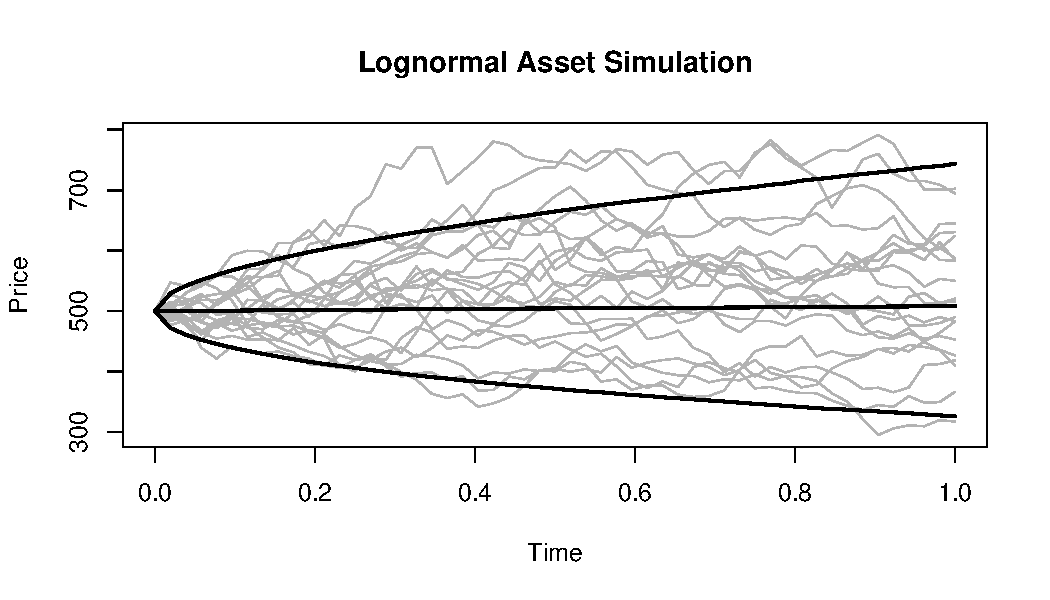
\includegraphics[scale=0.8]{../plots/q3/path_sim.pdf}
\caption{A sample of 20 from a total of $10^5$ total lognormal price processes generated for our underlying asset, with the mean and 95\% two-tailed confidence interval at each monitoring point plotted in black.}
\label{fig:path_sim}
\end{figure}

\indent We now consider the price of a geometric Asian call option written on the above asset, whose price has a known analytic form. Table \ref{tab:geo_asian_call_est} shows the results of the simulation of $N$ random variates for a crude estimator and $N/2$ variates for an antithetic estimator of the price option. Figures \ref{fig:geo_asian_call_sim}, \ref{fig:geo_asian_call_CI_time}, and \ref{fig:geo_asset_time_eff} visualizes this information, showing the convergence towards the analytic price for increasing $N$. We note that the antithetic estimator is more efficiency than the crude estimator for all $N$.

{\footnotesize
\csvautolongtable[
	table head=\caption{Geometric Asian call option value written on the underlying asset described above.}\label{tab:geo_asian_call_est}\\\hline
               \csvlinetotablerow\\\hline
               \endfirsthead\hline
               \csvlinetotablerow\\\hline
               \endhead\hline
               \endfoot,
               respect all
               ]{../data/q3_geo_clean_estimators.csv}
}

\begin{figure}[H]
	\centering
 	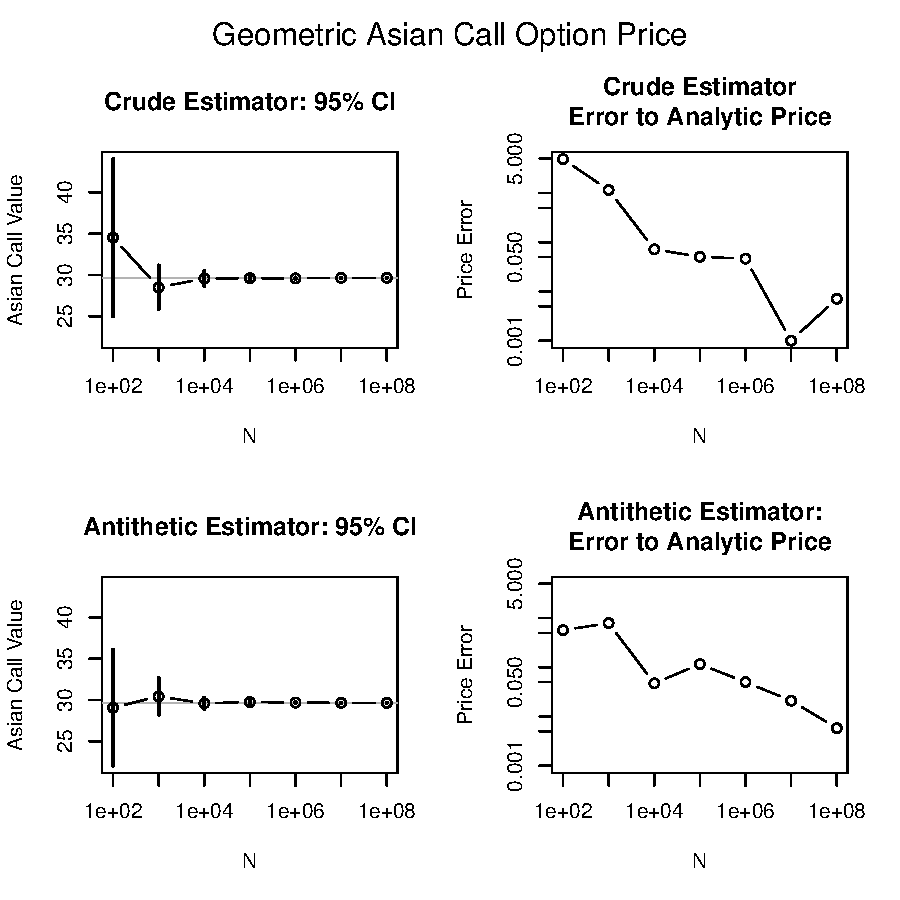
\includegraphics[scale=1]{../plots/q3/geo_asian_call_sim_est.pdf}
\caption{(Top) Crude simulation of a geometric Asian call option written on the above asset. (Bottom) Antithetic simulation of the same geometric Asian call. Note the convergence towards the true price (gray line) with increasing $N$.}
\label{fig:geo_asian_call_sim}
\end{figure}

\begin{figure}[H]
	\centering
 	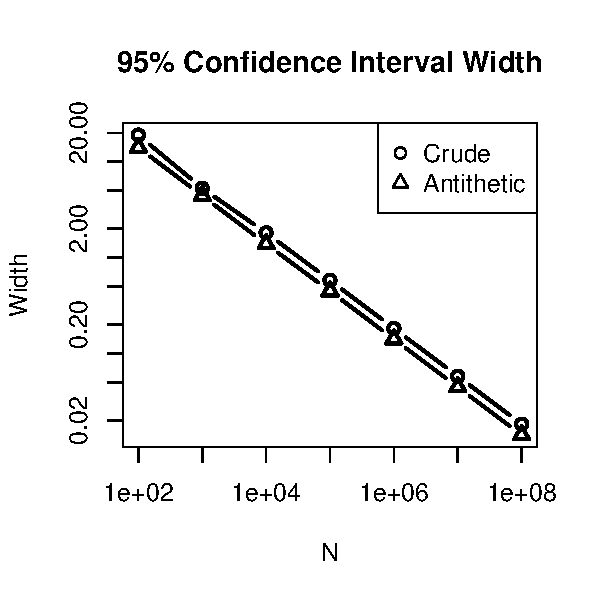
\includegraphics[scale=0.75]{../plots/q3/geo_asian_call_CI_widths.pdf}
	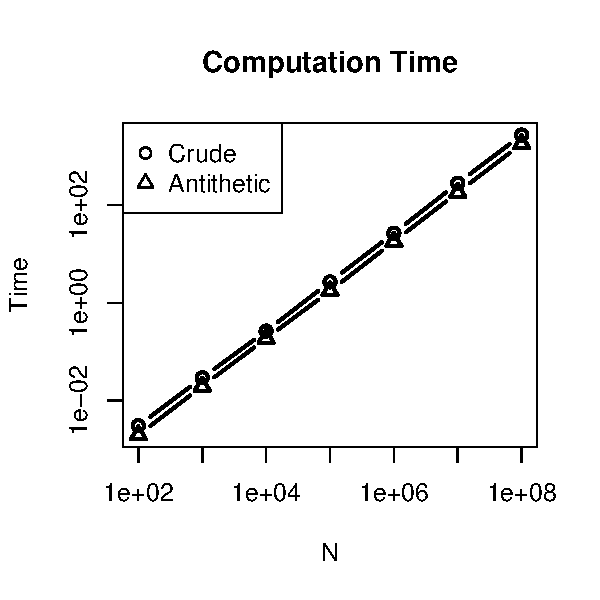
\includegraphics[scale=0.75]{../plots/q3/geo_asian_call_time.pdf}
\caption{Geometric Asian call option: (Left) Confidence intervals tighten for both crude and antithetic estimators at approximately the same (linear) rate. The antithetic estimator has a persistently narrower interval. (Right) Computation time increases linearly as a function of $N$ for both crude and antithetic estimators.}
\label{fig:geo_asian_call_CI_time}
\end{figure}
\begin{figure}[H]
	\centering
	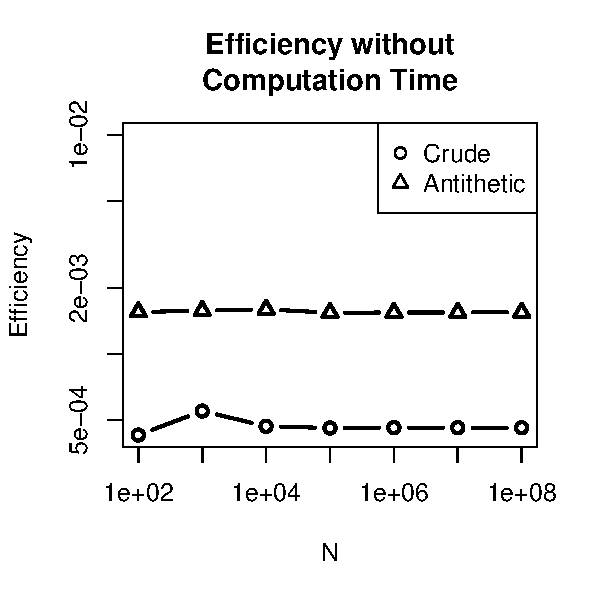
\includegraphics[scale=0.75]{../plots/q3/geo_asian_call_eff_wo_time.pdf}
\caption{Geometric Asian call option: The antithetic estimator is persistently more efficient than the crude estimator for all $N$.}
\label{fig:geo_asset_time_eff}
\end{figure}

\indent We now consider the same simulation for the price of an arithmetic Asian call option, which has no known analytic solution. In addition to the $N$ crude and $N/2$ antithetic random variates, we also introduce a control variate estimator for the arithmetic Asian option using the geometric Asian option price, whose expected value has an analytic solution. That is, we use the control variate
\begin{equation*}
	X_{Control} = X - c \left( Y - \mathbb E\left [ Y \right] \right)
\end{equation*}
such that $X$ is our arithmetic Asian call price, $Y$ the geometric Asian call price, $\mathbb E[Y]$ the analytic solution for the geometric Asian call, and the optimal $c$, denoted $c^*$, is found by
\begin{align*}
	c^* = -\frac{ \mathrm{Cov}[X, Y] }{ \mathrm{Var}[Y] }
\end{align*}

\indent For the control variate estimator we first pilot $m = 0.1\cdot N$ simulation to estimate the optimal $c^*$. Using this $c^*$ we then run the remaining $M = (N - m)$ simulations to estimate the arithmetic Asian call price itself. Table \ref{tab:ari_asian_call_est} shows the results of the simulation of $N$ crude variates, $N/2$ antithetic variates, and $0.9 \cdot N$ control variates. Figures \ref{fig:ari_asian_call_sim_est}, \ref{fig:ari_asian_call_CI_time}, and \ref{fig:ari_asset_time_eff} visualizes this information, showing the convergence towards the analytic price for increasing $N$. We note that while the antithetic estimator is more efficient than the crude estimator, the control variate estimator is profoundly more efficient than the other two.

{\footnotesize
\csvautolongtable[
	table head=\caption{Arithmetic Asian call option value written on the underlying asset described above.}\label{tab:ari_asian_call_est}\\\hline
               \csvlinetotablerow\\\hline
               \endfirsthead\hline
               \csvlinetotablerow\\\hline
               \endhead\hline
               \endfoot,
               respect all
               ]{../data/q3_clean_estimators.csv}
}

\begin{figure}[H]
	\centering
 	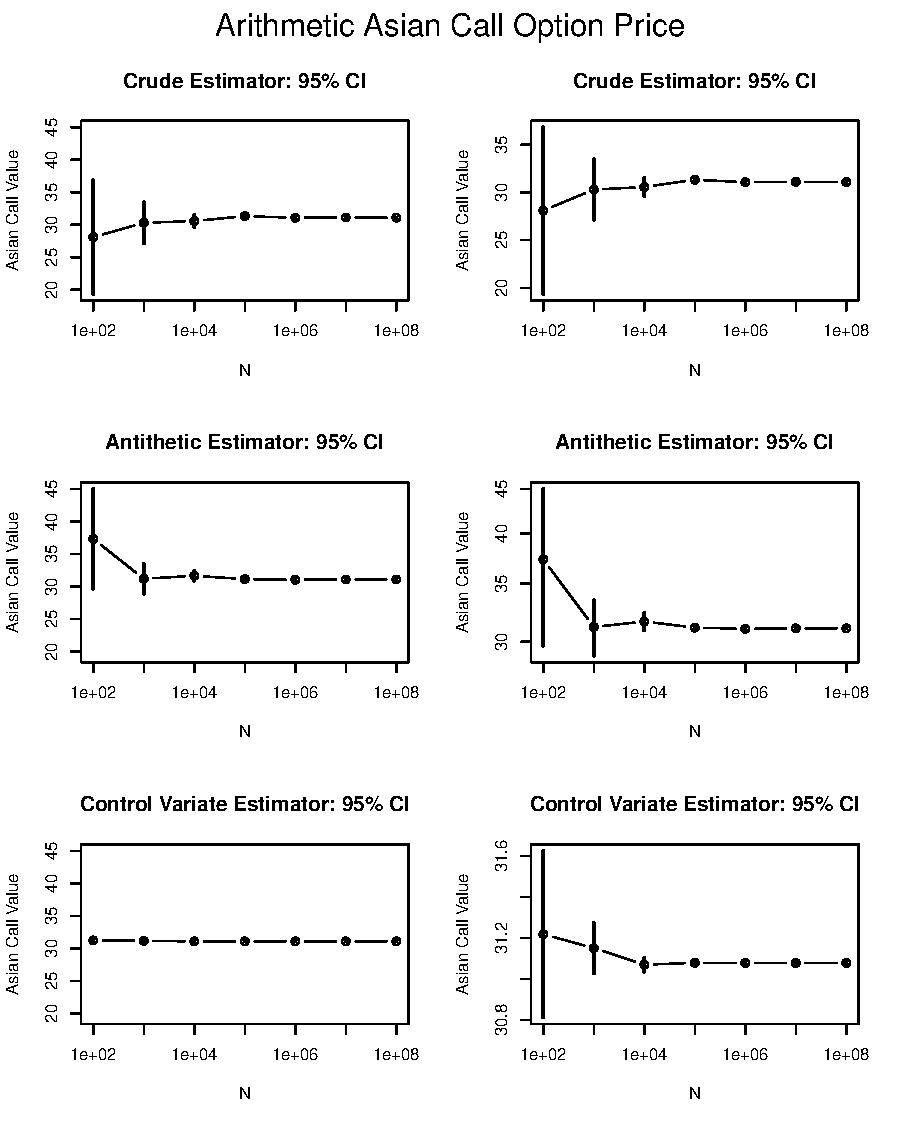
\includegraphics[scale=1]{../plots/q3/ari_asian_call_sim_est.pdf}
\caption{Arithmetic Asian call option: (Top) Crude simulation of a arithmetic Asian call option written on the above asset. (Middle) Antithetic simulation of the same arithmetic Asian call. (Bottom) Control variate simulation of the arithmetic Asian call.}
\label{fig:ari_asian_call_sim_est}
\end{figure}

\begin{figure}[H]
	\centering
 	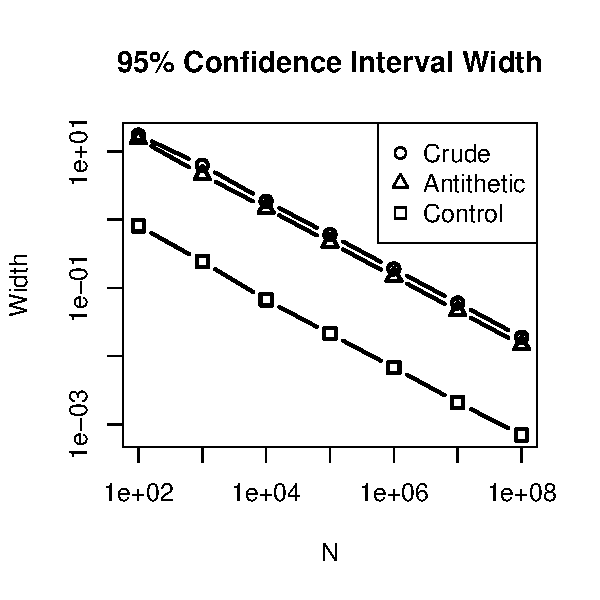
\includegraphics[scale=0.75]{../plots/q3/ari_asian_call_CI_widths.pdf}
	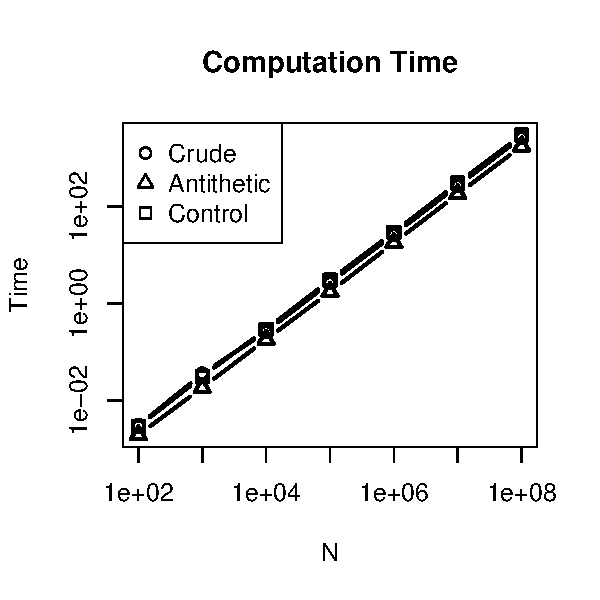
\includegraphics[scale=0.75]{../plots/q3/ari_asian_call_time.pdf}
\caption{Arithmetic Asian call option: (Left) Confidence interval widths tighten linearly with increasing $N$. Note the dramatic reduction in width using the control variate estimator. (Right) Computation time increases linearly as a function of $N$ for all estimators.}
\label{fig:ari_asian_call_CI_time}
\end{figure}
\begin{figure}[H]
	\centering
	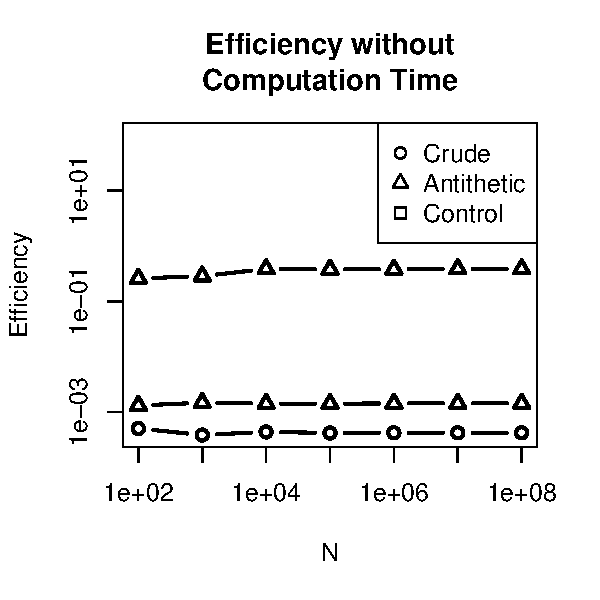
\includegraphics[scale=0.75]{../plots/q3/ari_asian_call_eff_wo_time.pdf}
\caption{Arithmetic Asian call option: Although the antithetic variate is persistently more efficient than the crude estimator, we see a dramatic increase in efficiency using the control variate estimator.}
\label{fig:ari_asset_time_eff}
\end{figure}


\newpage
\section{Question 4: {\normalfont Heston Stochastic Volatility Model}}

We wish to simulate an asset using the Heston stochastic volatility model
\begin{align*}
	dS_t &= rS_t\,dt + \sqrt{v_t}S_t\left[\rho\,dB^{(1)}_t + \sqrt{1 - \rho^2}\,dB^{(2)}_t \right] \\
	dv_t &= \kappa(\theta - v_t)\,dt + \sigma\sqrt{v_t}\,dB^{(1)}_t
\end{align*}

\indent We generate paths from the Heston model such that $S_0 = 100, v_0 = 0.1, T = 0.5$, and $n = 125$ discretization points using an Euler-discretization. Figure \ref{fig:heston_sample} shows us a sample of 20 paths (from $10^4$ total simulated paths) generated from the discretization of the Heston model. Using the same volatility process and identical Brownian increments we see the sample price processes for different $\rho$, in addition the sample means and the 95\% two-tailed confidence intervals at each discretized point.

\begin{figure}[H]
	\centering
	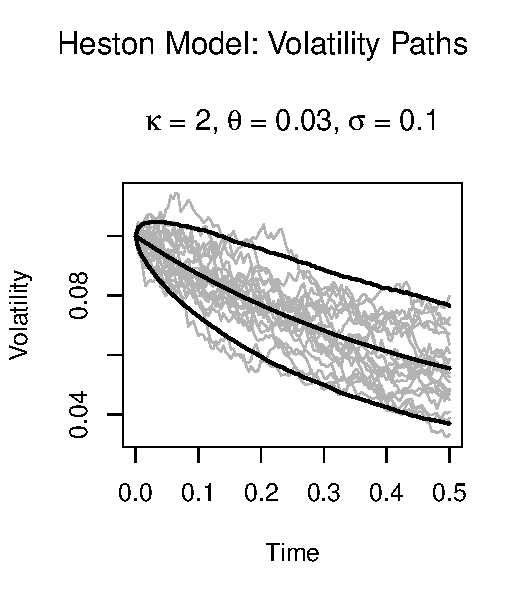
\includegraphics[scale=0.85]{../plots/q4/heston_sample_vols.pdf}
	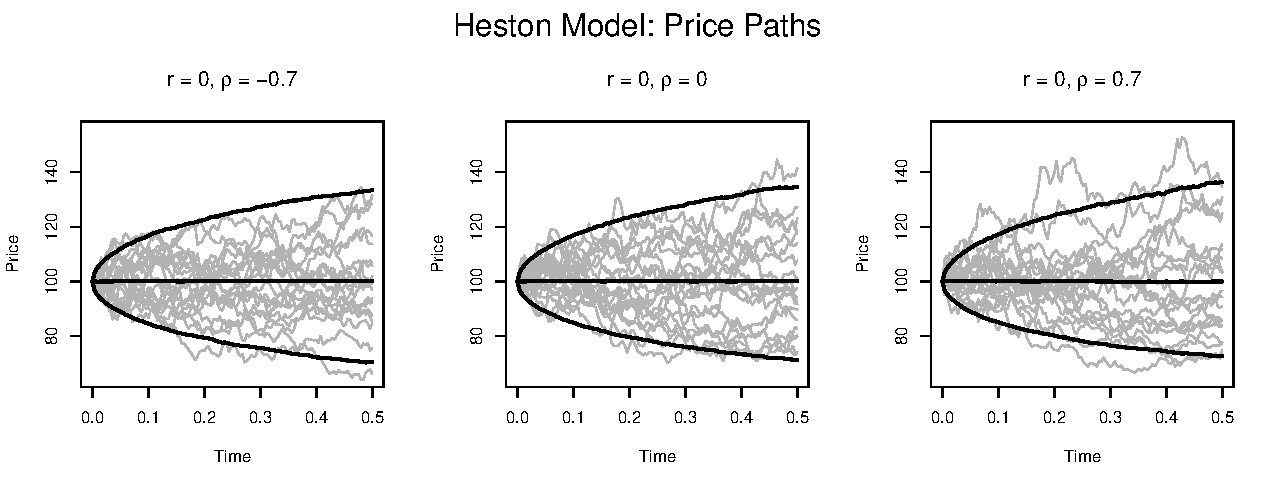
\includegraphics[scale=0.85]{../plots/q4/heston_sample_prices.pdf}
\caption{(Top) A sample of 20 from $10^4$ total volatility processes. (Bottom) A sample of 20 from a total of $10^4$ total price processes for different values of $\rho$. Means and 95\% two-tailed confidence intervals are also plotted (black) at each discretized point.}
\label{fig:heston_sample}
\end{figure}

\subsection{{\normalfont European Call Value -- Crude Estimator}}

\indent With our discretized price process in place we wish to find the value of a European call option with strike price $K = S_0 = 100$. We first use a crude estimator to determine its value. Table \ref{tab:heston_crude_call_est} shows the results of the simulation of $N$ random variates for a crude estimator. We visualize this information below in Figure \ref{fig:heston_call_est} when comparing the results to that of the conditional estimator.

{\footnotesize
\csvautolongtable[
	table head=\caption{Crude estimator of the value of a European call option written on an underlying asset with dynamics described by the Heston stochastic volatility model above.}\label{tab:heston_crude_call_est}\\\hline
               \csvlinetotablerow\\\hline
               \endfirsthead\hline
               \csvlinetotablerow\\\hline
               \endhead\hline
               \endfoot,
               respect all
               ]{../data/q4a_clean_heston_crude_est.csv}
}

\subsection{{\normalfont European Call Value -- Conditional Estimator}}

\indent Similar to the crude estimator, we now wish to find the price of a European call option with strike price $K = S_0 = 100$ on the above asset using a conditional Monte-Carlo estimator. To implement a conditional Monte-Carlo estimator we use the following result
\begin{equation*}
	\mathbb E_{\mathbb Q} \left[e^{-rT} \left(S_T - K\right)^+ \Big| \left\{B^{(1)}_t: 0 \leq t \leq T \right\} \right]  = S_0 \xi \Phi(\tilde{d_1}) - Ke^{-rT}\Phi(\tilde{d_2})
\end{equation*}

where
\begin{align*}
	\xi &= \exp \left( -\frac{\rho^2}{2} \int^T_0 v_t\,dt + \rho \int^T_0 \sqrt{v_t}\,dB^{(1)}_t \right) \\
	\tilde{d_1} &= \frac{ \log \frac{S_0\xi}{K} + \left(r + \frac{1}{2}\tilde{\sigma}^2 \left(1 - \rho^2 \right)\right) }{ \tilde{\sigma}\sqrt{T(1 - \rho^2)} } \\
	\tilde{d_2} &= \tilde{d_1} - \tilde{\sigma}\sqrt{T(1 - \rho^2)} \\
	\tilde{\sigma}^2 &= \frac{1}{T} \int^T_0 v_t \,dt
\end{align*}

\indent With this estimator we wish to find the value of a European call option written on the asset described by the same Heston process. Table \ref{tab:heston_cmc_call_est} shows the results of the simulation of $N$ random variates for a the conditional Monte-Carlo estimator.

{\footnotesize
\csvautolongtable[
	table head=\caption{Conditional Monte-Carlo estimator of the value of a European call option written on the underlying asset with dynamics described by the Heston stochastic volatility model above.}\label{tab:heston_cmc_call_est}\\\hline
               \csvlinetotablerow\\\hline
               \endfirsthead\hline
               \csvlinetotablerow\\\hline
               \endhead\hline
               \endfoot,
               respect all
               ]{../data/q4b_clean_heston_cmc_est.csv}
}

\subsection{{\normalfont Crude and Conditional Estimator Comparison}}

\indent We now take a moment to visualize the data in Tables \ref{tab:heston_crude_call_est} and \ref{tab:heston_cmc_call_est} in order to compare the performance of both European call estimators in the Heston model. Figures \ref{fig:heston_call_est}, \ref{fig:heston_call_CI} and \ref{fig:heston_call_time_eff} show us the convergence for the value of the European call option with increased $N$ over the three values for $\rho$. Of note is the superiority of the conditional Monte-Carlo estimator made apparent in Figures \ref{fig:heston_call_CI} and \ref{fig:heston_call_time_eff}: The conditional estimator is consistently more efficient than its crude sibling. Furthermore, the conditional estimator requires less computational effort than its crude counterpart since, while the crude estimator requires the simulation of the price process (thereby requiring the volatility process), the conditional estimator only requires the simulation of the volatility process.

\begin{figure}[H]
	\centering
 	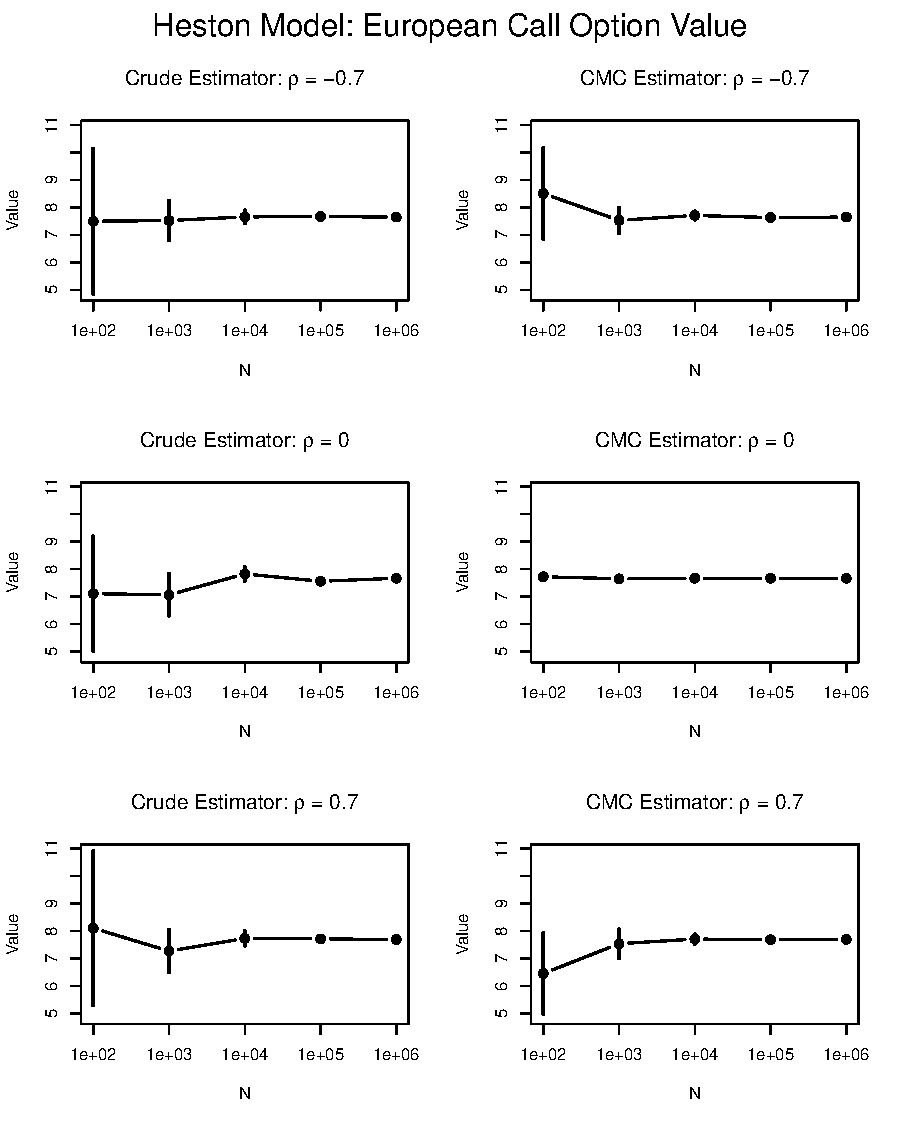
\includegraphics[scale=1]{../plots/q4/heston_call_est.pdf}
\caption{(Left) Crude and (Right) conditional Monte-Carlo simulations for the value of a European call option written on an underlying asset following the Heston stochastic volatility model.}
\label{fig:heston_call_est}
\end{figure}

\begin{figure}[H]
	\centering
 	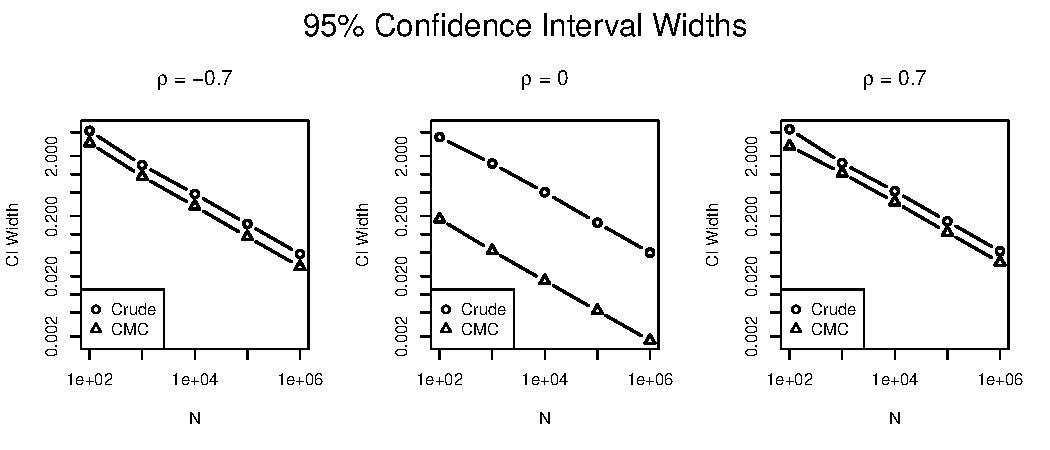
\includegraphics[scale=1]{../plots/q4/heston_call_CI_width.pdf}
\caption{Comparison of the 95\% confidence intervals generated by the crude and conditional Monte-Carlo estimators given various values for $\rho$. Note the persistent reduction in interval width by using the conditional estimator, with a profound reduction when $\rho = 0$.}
\label{fig:heston_call_CI}
\end{figure}

\begin{figure}[H]
	\centering
 	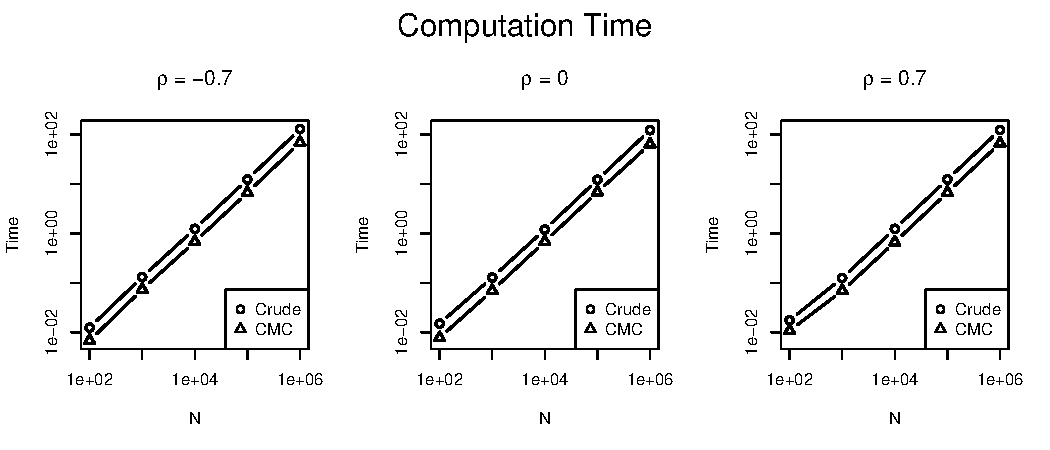
\includegraphics[scale=1]{../plots/q4/heston_call_time.pdf}
 	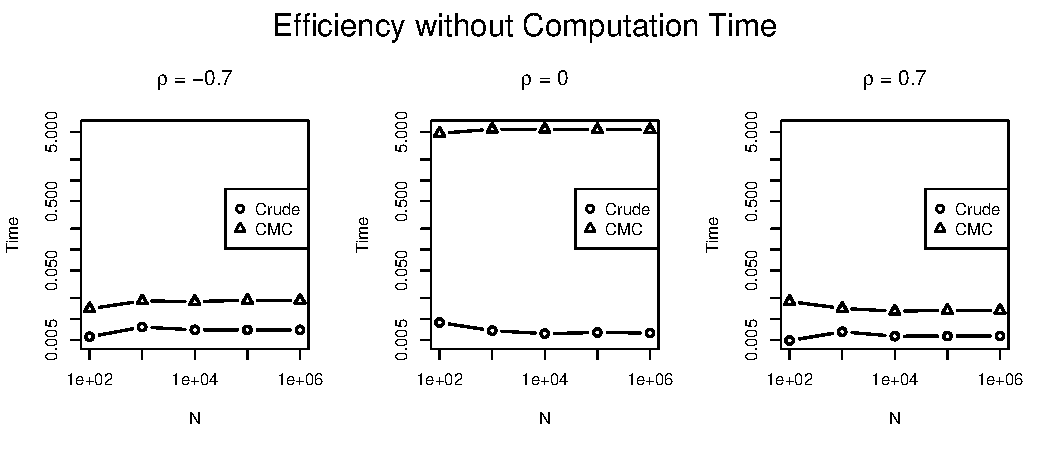
\includegraphics[scale=1]{../plots/q4/heston_call_eff.pdf}
\caption{Comparison of the (Top) computation time and (Bottom) estimator efficiency for the crude and conditional Monte-Carlo estimators. Of interest is the increased efficiency of the conditional Monte-Carlo estimator which is particularly apparent when $\rho = 0$.}
\label{fig:heston_call_time_eff}
\end{figure}






\newpage
\appendix
\section{Code}
\subsection{main\_q1.cpp}
\lstinputlisting{../code/q1/main_q1.cpp}

\subsection{main\_q3.cpp}
\lstinputlisting{../code/q3/main_q3.cpp}

\subsection{main\_q4a.cpp}
\lstinputlisting{../code/q4a/main_q4a.cpp}

\subsection{main\_q4b.cpp}
\lstinputlisting{../code/q4b/main_q4b.cpp}

\subsection{MathHelp.h}
\lstinputlisting{../code/q4b/MathHelp.h}
\subsection{MathHelp.cpp}
\lstinputlisting{../code/q4b/MathHelp.cpp}

\subsection{rng.h}
\lstinputlisting{../code/q4b/rng.h}
\subsection{rng.cpp}
\lstinputlisting{../code/q4b/rng.cpp}

\subsection{Asset.h}
\lstinputlisting{../code/q4b/Asset.h}
\subsection{Asset.cpp}
\lstinputlisting{../code/q4b/Asset.cpp}

\subsection{HestonAsset.h}
\lstinputlisting{../code/q4b/HestonAsset.h}
\subsection{HestonAsset.cpp}
\lstinputlisting{../code/q4b/HestonAsset.cpp}

\subsection{Option.h}
\lstinputlisting{../code/q4b/Option.h}
\subsection{Option.cpp}
\lstinputlisting{../code/q4b/Option.cpp}

\subsection{VanillaOption.h}
\lstinputlisting{../code/q4b/VanillaOption.h}
\subsection{VanillaOption.cpp}
\lstinputlisting{../code/q4b/VanillaOption.cpp}

\subsection{AsianOption.h}
\lstinputlisting{../code/q4b/AsianOption.h}
\subsection{AsianOption.cpp}
\lstinputlisting{../code/q4b/AsianOption.cpp}

\subsection{AriAsianOption.h}
\lstinputlisting{../code/q4b/AriAsianOption.h}
\subsection{AriAsianOption.cpp}
\lstinputlisting{../code/q4b/AriAsianOption.cpp}

\subsection{GeoAsianOption.h}
\lstinputlisting{../code/q4b/GeoAsianOption.h}
\subsection{GeoAsianOption.cpp}
\lstinputlisting{../code/q4b/GeoAsianOption.cpp}




































\end{document}